\documentclass[a4paper, 12pt]{report}
\usepackage{booktabs}
\usepackage{graphicx}
\usepackage[table]{xcolor}
\usepackage{tabularx}
\usepackage[utf8]{inputenc}
\usepackage{multirow} % Pour fusionner les cellules sur plusieurs lignes
\usepackage[french]{babel}
\usepackage{underscore}
\usepackage[T1]{fontenc}
\usepackage{tikz}
\usepackage{graphicx} % Package pour gérer les images
% Préambule (packages, configurations, etc.)
\usepackage[utf8]{inputenc} % Encodage du texte en UTF-8
\usepackage[T1]{fontenc}    % Encodage des polices en T1 (accents, etc.)
\usepackage{tcolorbox}
\usepackage{xcolor} % Pour la gestion des couleurs
\usepackage{titlesec} % Pour personnaliser le style des sections
\usepackage{ragged2e}
\usepackage{geometry}
\usepackage{fancyhdr}
\usepackage{tabularx}
\usepackage{booktabs}
\usepackage{float}
\usepackage[
    hidelinks
]{hyperref}
\geometry{
    a4paper,
    total={170mm,257mm},
    left=25mm,
    top=30mm,
     bottom=25mm % Ajuster la marge inférieure
}
\setlength{\parskip}{1ex plus 0.5ex minus 0.2ex}
\usepackage{amsmath}
\usepackage{amssymb}
\usepackage{enumitem}
\usepackage{caption}
\usepackage{longtable}
\usepackage[french, capitalise, nameinlink]{cleveref}
%\counterwithin{figure}{part} % Numéroter les figures selon la section
%\counterwithin{table}{part}
% Définition du format des titres de partie

% Définition du format des titres de partie
\titleformat{\part}[display]
  {\normalfont\huge\bfseries\color{subtitle}}
  {\partformat}
  {0pt}
  {\Huge}

\newcommand{\rapportEntreprise}{[Nom de l'organisme d'accueil]} % À ADAPTER
% Format pour le numéro de partie
\newcommand{\partformat}{Chapitre \thepart}

% Changer la numérotation des parties
\renewcommand{\thepart}{\arabic{part}}




\DeclareCaptionFormat{customformat}{\textbf{{#1#2}}#3}
\captionsetup[figure]{format=customformat}

\DeclareCaptionFormat{tablecustomformat}{\textbf{{#1#2}}#3}
\captionsetup[table]{format=tablecustomformat}

% Définition des couleurs personnalisées
\definecolor{customcolor}{HTML}{ED6E0A}
\definecolor{subtitle}{HTML}{047F64}
\definecolor{subtitle1}{HTML}{0077b6}
\definecolor{tablegray}{gray}{0.7}

% Personnalisation du style des titres de section
\titleformat*{\section}{\fontsize{20}{25}\selectfont\bfseries}
\titleformat*{\subsection}{\Large\bfseries}
\titleformat*{\subsubsection}{\large\bfseries}
\setcounter{secnumdepth}{3}

\usepackage{listings}

\definecolor{codebg}{HTML}{F5F5F5}
\definecolor{codekeyword}{HTML}{0057AE}
\definecolor{codecomment}{HTML}{6A9955}
\definecolor{codestring}{HTML}{A31515}

\lstdefinestyle{monstyle}{
    backgroundcolor=\color{codebg},
    commentstyle=\color{codecomment}\itshape,
    keywordstyle=\color{codekeyword}\bfseries,
    stringstyle=\color{codestring},
    basicstyle=\ttfamily\small,
    breaklines=true,
    frame=single,
    rulecolor=\color{gray!50},
    numbers=left,
    numberstyle=\tiny\color{gray},
    numbersep=8pt,
    showstringspaces=false,
    xleftmargin=15pt,
    framexleftmargin=15pt,
}
\lstset{style=monstyle}

\usepackage{graphicx} % Assurez-vous que ce package est inclus dans le préambule
\usetikzlibrary{positioning}
% Configuration du format des titres de chapitre
\usepackage{titlesec}
\titleformat{\chapter}[display]{\normalfont\huge\bfseries}{Chapitre \thechapter}{20pt}{\Huge}
\usepackage{graphicx} % Assurez-vous que ce package est inclus dans le préambule
\titlespacing*{\chapter}{0pt}{2.52pt}{2.52pt}
% Informations sur le document
\title{\textbf{Rapport de Projet de Fin d'Études}}

\author{Réalisé par: \\
        Fatma Chahed  }
\date{ Date: \today}
% ===================== MÉTADONNÉES ===================== % À ADAPTER
\newcommand{\Universite}{Université de Tunis El Manar} % À ADAPTER
\newcommand{\Departement}{Département Informatique} % À ADAPTER
\newcommand{\Matiere}{Génie logiciel / Systèmes d'information géographique}
\newcommand{\Intitule}{Conception et modélisation d'une plateforme de géolocalisation des biens immobiliers en Tunisie}
\newcommand{\SousIntitule}{}
\newcommand{\SousTitre}{Rapport de Projet de Fin d'Études}
\newcommand{\Etudiante}{Fatma CHAHED} % À ADAPTER
\newcommand{\Encadranted}{Mme./M. [Encadrant académique]} % À ADAPTER
\newcommand{\Encadrantew}{Mme./M. [Encadrant professionnel]} % À ADAPTER
\newcommand{\Annee}{2025--2026}
\newcommand{\titreintro}[1]{%
    \vspace{1em}
    \noindent
    {\LARGE\bfseries #1}
    \vspace{0.5em}
}

\begin{document}
% ----------- PAGE DE GARDE -----------
\thispagestyle{empty}
\begin{center}
    \noindent
    \begin{minipage}{0.48\textwidth}
        \raggedright
            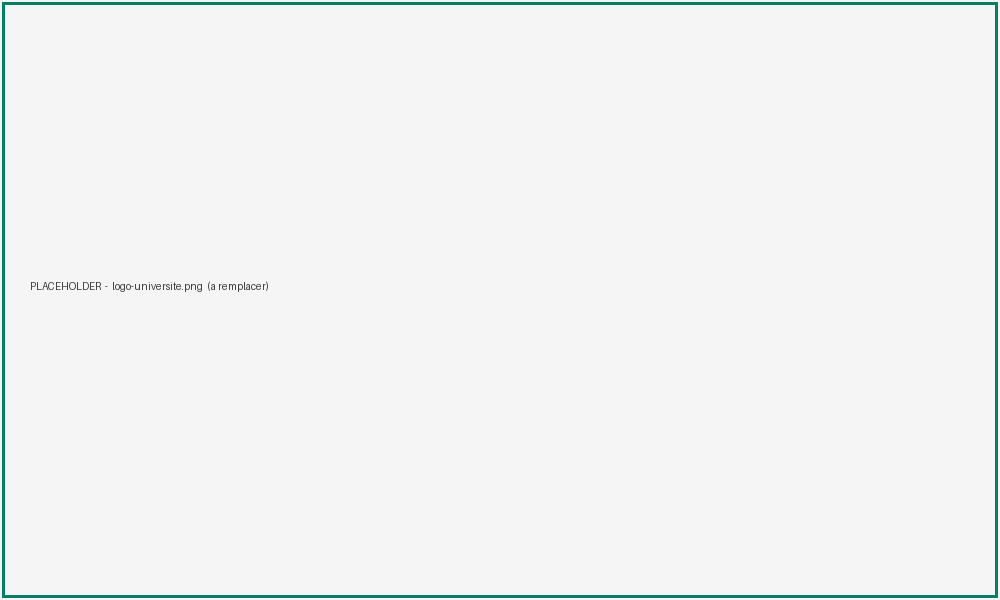
\includegraphics[height=3.5cm]{images/logo-universite.png} % À FOURNIR
    \end{minipage}
    \hfill
    \begin{minipage}{0.4\textwidth}
        \raggedleft
            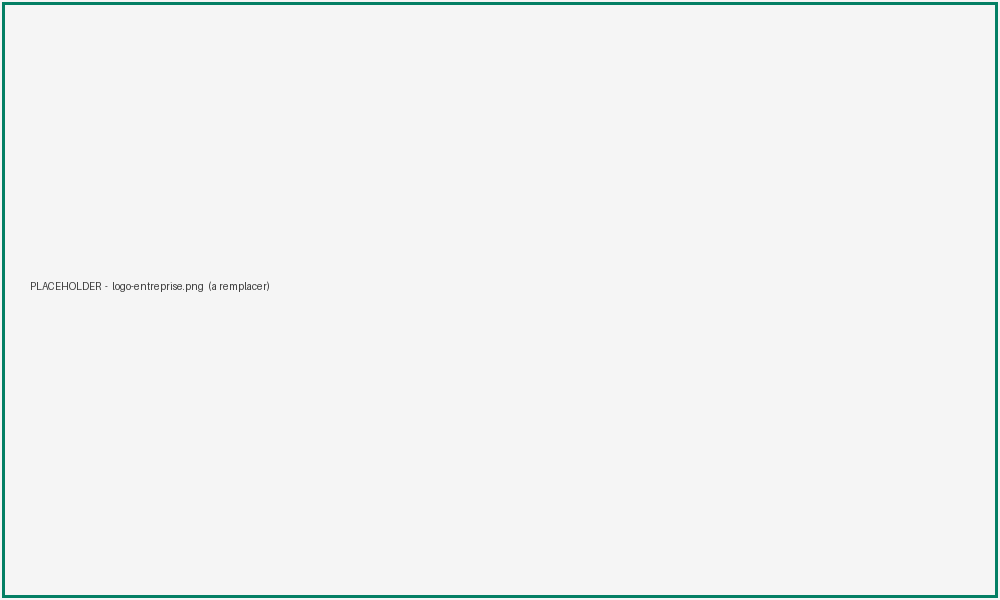
\includegraphics[height=1.8cm]{images/logo-entreprise.png} % À FOURNIR
    \end{minipage}

    \vspace{0.8cm}
    {\Large \textbf{Projet de Fin d'Études pour l'obtention du diplôme de [Licence / Mastère] en Informatique}}\\[0.25cm]
    {\large \Universite}\\[1cm]
    {\large\textbf{Année universitaire :} \Annee\\[6pt]}
\end{center}

% ----------- TITRE ENTRE DEUX FILETS HORIZONTAUX (sans cadre) -----------
\vspace{0.2cm}
\begin{center}
    {\rule{\linewidth}{1.2pt}}\\[0.9cm]
    {\huge\bfseries\Intitule\par}
    \vspace{0.35cm}
    {\huge\bfseries\SousIntitule\par}
    \vspace{0.9cm}
    {\Large\bfseries \SousTitre\par}
    \vspace{0.9cm}
    {\rule{\linewidth}{1.2pt}}
\end{center}

% ----------- BLOC INFOS : Étudiante à gauche, Encadrantes à droite -----------
\vspace{1.2cm}
\noindent\makebox[\linewidth]{%
  \begin{minipage}[t]{0.42\linewidth}
    \raggedright
    {\large\textbf{Élaboré par :}}\\[8pt]
    {\large \Etudiante}\\[15pt]
    {\large\textbf{Au sein de :}}\\[8pt]
    {\large \rapportEntreprise}\\[15pt]
    % {\large\textbf{Année universitaire :}}\\[8pt]
    % {\large 2025 / 2026}
  \end{minipage}%
  \hspace{0.14\linewidth}% <-- espace entre l'étudiante et les enseignantes
  \begin{minipage}[t]{0.42\linewidth}
    \raggedleft
    {\large\textbf{Encadrant académique  :}}\\[8pt]
    {\large \Encadranted}\\[15pt]
    {\large\textbf{Encadrant professionnel :}}\\[8pt]
    {\large \Encadrantew}
  \end{minipage}%
}


% ----------- LIMINAIRES -----------
\pagenumbering{roman}
\section*{ \centering Dédicaces }


À ma \textbf{chère mère}, qui m'a toujours encouragée et poussée à atteindre mes objectifs, je suis infiniment reconnaissante pour ta présence aimante et ton soutien indéfectible.
\vspace{0.5cm}

À mon \textbf{cher père}, qui a toujours été là pour m'aider à surmonter les difficultés, je suis profondément reconnaissante pour ta présence rassurante et ton soutien inébranlable.
\vspace{0.5cm}

À ma \textbf{famille} et à mes \textbf{amis les plus proches}, pour leur soutien constant et leurs encouragements tout au long de ce parcours.
\vspace{0.5cm}

À toutes les personnes qui, de près ou de loin, ont contribué à la réussite de ce travail.


Avec toute ma reconnaissance,


\begin{flushright}
\textbf{\Etudiante}
\end{flushright}

\newpage
\section* {\centering Remerciements }
Ce travail n'aurait pas été mené à bien sans l'aide et le soutien de plusieurs personnes auxquelles je tiens à exprimer ma plus profonde gratitude.

Je remercie tout d'abord mon encadrant académique, \textbf{\Encadranted}, pour sa disponibilité, ses conseils avisés et son accompagnement rigoureux tout au long de ce projet.

Je remercie également mon encadrant professionnel, \textbf{\Encadrantew}, ainsi que l'ensemble de l'équipe de \textbf{\rapportEntreprise}, pour leur accueil, leur confiance et les moyens mis à ma disposition durant la période de stage.

Mes remerciements s'adressent aussi aux membres du jury qui ont accepté d'évaluer ce travail, ainsi qu'à tout le corps enseignant de \Universite\ pour la qualité de la formation dispensée.

Enfin, je remercie ma famille et mes amis pour leur soutien indéfectible.
\vspace{1cm}

\begin{flushright}
\textbf{\Etudiante}
\end{flushright}

% --- Table des matières ---
\renewcommand{\contentsname}{Table des matières}
\tableofcontents

\renewcommand{\listfigurename}{Table des figures}
\listoffigures

\renewcommand{\listtablename}{Liste des tableaux}
\listoftables

\newpage
\section*{ \centering Liste des acronymes}
\begin{itemize}
    \item[--] \textbf{UML :} Unified Modeling Language
    \item[--] \textbf{UI :} User Interface (interface utilisateur)
    \item[--] \textbf{UX :} User Experience (expérience utilisateur)
    \item[--] \textbf{MCD :} Modèle Conceptuel de Données
    \item[--] \textbf{MLD :} Modèle Logique de Données
    \item[--] \textbf{SGBD :} Système de Gestion de Base de Données
    \item[--] \textbf{SIG :} Système d'Information Géographique
    \item[--] \textbf{GPS :} Global Positioning System
    \item[--] \textbf{OSM :} OpenStreetMap
    \item[--] \textbf{API :} Application Programming Interface
    \item[--] \textbf{CU :} Cas d'Utilisation
    \item[--] \textbf{RGPD :} Règlement Général sur la Protection des Données
    \item[--] \textbf{WCAG :} Web Content Accessibility Guidelines
\end{itemize}
\newpage

% --- Résumé (page à part, avec un vrai titre) ---
\newpage
\section*{\centering Résumé}
Ce rapport porte sur la \textbf{conception et la modélisation} d'une plateforme web
de \textbf{géolocalisation des biens immobiliers en Tunisie}, destinée à mettre en
relation particuliers, agences et promoteurs autour d'annonces immobilières
localisées sur une carte interactive.

Le travail couvre exclusivement la phase amont~: étude du contexte et des besoins,
formalisation du cahier des charges, \textbf{modélisation UML} (diagrammes de cas
d'utilisation, de classes et de séquence), \textbf{conception de la base de
données} (modèle conceptuel, modèle logique et dictionnaire de données), puis
\textbf{conception des interfaces utilisateur} selon une démarche UX/UI sous Figma
(arborescence, wireframes, charte graphique, maquettes et prototype interactif).

La contribution principale réside dans la définition d'un modèle de données
structuré autour du découpage administratif tunisien (gouvernorat, délégation,
localité) couplé à des coordonnées géographiques précises (latitude, longitude),
et dans la conception d'un parcours utilisateur centré sur la recherche
cartographique.

\vspace{1.5em}
\noindent\textbf{Mots-clés~:} géolocalisation, biens immobiliers, Tunisie, conception, modélisation UML, base de données, SIG, cartographie, UX/UI, Figma, maquettage.
\clearpage

\pagenumbering{arabic}

% =================== CORPS DU RAPPORT ===================

\chapter{Introduction générale}
\label{chap:intro}
% ===================== INTRODUCTION GÉNÉRALE =====================

Le marché immobilier tunisien reste largement structuré autour d'annonces
diffusées sur des sites généralistes, où la localisation d'un bien se résume le
plus souvent à un nom de ville ou de quartier saisi librement. Cette imprécision
rend la recherche fastidieuse pour l'acquéreur ou le locataire, qui ne peut ni
visualiser la répartition géographique de l'offre, ni filtrer autour d'un point
d'intérêt (lieu de travail, école, transport).

Le présent projet, réalisé au sein de \rapportEntreprise, vise à concevoir une
plateforme web dédiée à la \textbf{géolocalisation des biens immobiliers en
Tunisie}. Chaque bien y est positionné précisément sur une carte interactive,
rattaché au découpage administratif national (gouvernorat, délégation, localité)
et enrichi de coordonnées géographiques (latitude, longitude).

\paragraph{Problématique.}
\emph{Comment concevoir et modéliser une plateforme web permettant de publier,
géolocaliser et rechercher des biens immobiliers en Tunisie, de manière fiable et
ergonomique, en tenant compte des spécificités du découpage territorial
tunisien~?}

\paragraph{Objectif.}
Ce travail couvre exclusivement la \textbf{phase de conception}~: analyse du
contexte et des besoins, cahier des charges, modélisation UML (cas d'utilisation,
classes, séquence), conception de la base de données (MCD, MLD, dictionnaire de
données) et conception des interfaces sous Figma (arborescence, wireframes,
charte graphique, maquettes, prototype). La phase de développement n'entre pas
dans le périmètre de ce rapport.

\paragraph{Organisation du rapport.}
Le \textbf{chapitre~\ref{chap:contexte}} présente l'organisme d'accueil, l'étude
de l'existant, la problématique et le cahier des charges. Le
\textbf{chapitre~\ref{chap:solution}} introduit les concepts clés et la solution
proposée. Le \textbf{chapitre~\ref{chap:conception}} détaille la modélisation du
système et de la base de données. Le \textbf{chapitre~\ref{chap:uxui}} présente
la conception des interfaces utilisateur. Une conclusion dresse le bilan et
ouvre des perspectives.


\chapter{Contexte général}
\label{chap:contexte}
% ===================== CHAPITRE 1 : CONTEXTE GÉNÉRAL =====================

\section*{Introduction}
Ce chapitre situe le projet~: présentation de l'organisme d'accueil, analyse de
l'existant, formulation de la problématique et des objectifs, puis cahier des
charges.

\section{Présentation de l'organisme d'accueil}
\label{sec:organisme}

\begin{tcolorbox}[colback=codebg,colframe=subtitle,title=À compléter]
Section à rédiger avec les informations officielles de \rapportEntreprise\
(dénomination, forme juridique, création, effectif, activité, organigramme).
Le tableau ci-dessous sert de trame.
\end{tcolorbox}

\begin{table}[H]
\centering
\renewcommand{\arraystretch}{1.25}
\begin{tabularx}{\linewidth}{>{\bfseries}p{4cm} X}
\toprule
Raison sociale     & \rapportEntreprise \\
Forme juridique    & [SARL / SUARL / SA] \\
Date de création   & [\ldots] \\
Siège social       & [Adresse, gouvernorat] \\
Activité           & Édition de logiciels / services numériques \\
Effectif           & [\ldots] \\
\bottomrule
\end{tabularx}
\caption{Fiche d'identité de l'organisme d'accueil}
\label{tab:fiche-entreprise}
\end{table}

\section{Étude de l'existant}
\label{sec:existant}

La diffusion d'annonces immobilières en Tunisie repose sur des portails de
petites annonces généralistes, des sites d'agences et des réseaux sociaux.
L'analyse de ces solutions fait ressortir les limites suivantes~:

\begin{table}[H]
\centering
\renewcommand{\arraystretch}{1.25}
\begin{tabularx}{\linewidth}{>{\bfseries}p{4.2cm} X}
\toprule
Localisation approximative & Champ « ville » ou « quartier » en texte libre, sans position sur carte. \\
Recherche peu ergonomique  & Filtres limités, pas de recherche « autour de moi » ni par zone. \\
Découpage territorial ignoré & Le triplet gouvernorat / délégation / localité n'est pas exploité de façon structurée. \\
Qualité des annonces        & Doublons, annonces obsolètes, peu de modération. \\
Expérience mobile           & Interfaces non pensées « mobile-first ». \\
\bottomrule
\end{tabularx}
\caption{Limites des solutions existantes}
\label{tab:limites-existant}
\end{table}

\section{Problématique et objectifs}
\label{sec:problematique}

Il s'agit de concevoir une plateforme permettant de \emph{publier, géolocaliser
et rechercher} des biens immobiliers en Tunisie, en s'appuyant sur le découpage
territorial national et sur une carte interactive. Les objectifs sont~:

\begin{itemize}[label=\textbullet,itemsep=1pt]
  \item offrir une \textbf{recherche cartographique} fluide (déplacement, zoom,
        regroupement de marqueurs, recherche par zone)~;
  \item permettre la \textbf{publication géolocalisée} d'une annonce par
        placement d'un point sur la carte et géocodage inverse de l'adresse~;
  \item structurer les données autour du référentiel
        \textbf{gouvernorat $\rightarrow$ délégation $\rightarrow$ localité}~;
  \item gérer plusieurs \textbf{profils d'utilisateurs} et leurs droits~;
  \item proposer une expérience \textbf{responsive}, pensée pour le mobile.
\end{itemize}

\section{Cahier des charges}
\label{sec:cahier-des-charges}

\begin{table}[H]
\centering
\renewcommand{\arraystretch}{1.2}
\begin{tabularx}{\linewidth}{>{\bfseries}p{1.3cm} p{3.2cm} X}
\toprule
Réf. & Module & Description \\
\midrule
BF-01 & Comptes         & Inscription, connexion, profil, rôles. \\
BF-02 & Annonces        & Création, modification, suppression, publication. \\
BF-03 & Géolocalisation & Placement sur carte, latitude/longitude, géocodage inverse. \\
BF-04 & Référentiel géo. & Sélection gouvernorat / délégation / localité, recherche de lieu. \\
BF-05 & Recherche       & Filtres (catégorie, type, prix, surface, pièces\ldots), recherche sur carte. \\
BF-06 & Détail bien     & Fiche complète, galerie photos, carte de situation, contact. \\
BF-07 & Favoris \& alertes & Enregistrer un bien, sauvegarder une recherche, alerte de prix. \\
BF-08 & Comparateur     & Comparer plusieurs biens. \\
BF-09 & Espace agence   & Portefeuille d'annonces, agents, tableau de bord. \\
BF-10 & Modération      & Validation / refus des annonces, gestion des comptes (admin). \\
\bottomrule
\end{tabularx}
\caption{Besoins fonctionnels}
\label{tab:besoins-fonctionnels}
\end{table}

\begin{table}[H]
\centering
\renewcommand{\arraystretch}{1.2}
\begin{tabularx}{\linewidth}{>{\bfseries}p{3cm} X}
\toprule
Exigence & Description \\
\midrule
Ergonomie     & Interface claire, « mobile-first », conforme aux heuristiques de Nielsen. \\
Performance   & Affichage carte et résultats $<$ 2~s~; regroupement des marqueurs. \\
Portabilité   & Application web responsive, navigateurs récents. \\
Sécurité      & Authentification, contrôle d'accès par rôle. \\
Maintenabilité & Architecture en couches, modèle de données extensible. \\
Conformité    & Respect des principes du RGPD. \\
\bottomrule
\end{tabularx}
\caption{Besoins non fonctionnels}
\label{tab:besoins-non-fonctionnels}
\end{table}

\section*{Conclusion}
Le cadre du projet est posé~: contexte, existant, problématique et cahier des
charges. Le chapitre suivant présente la solution proposée.


\chapter{Solution proposée}
\label{chap:solution}
% ===================== CHAPITRE 2 : SOLUTION PROPOSÉE =====================

\section*{Introduction}
Ce chapitre présente les concepts clés du projet, décrit la solution proposée,
puis identifie les acteurs et les principaux cas d'utilisation.

\section{Concepts clés}
\label{sec:concepts}

\paragraph{Géolocalisation et géocodage.}
La \textbf{géolocalisation} consiste à déterminer la position d'un objet au moyen
de coordonnées géographiques (latitude, longitude) dans le système de référence
WGS~84. Le \textbf{géocodage inverse} convertit des coordonnées en une adresse
lisible~: lorsqu'un utilisateur place un marqueur sur la carte, le champ adresse
est ainsi pré-rempli automatiquement.

\paragraph{Cartographie web.}
L'affichage repose sur un fond de carte composé de \emph{tuiles} (issues
d'OpenStreetMap) sur lequel sont superposés des \emph{marqueurs}. Un mécanisme de
\emph{regroupement} (\emph{clustering}) agrège les marqueurs proches pour rester
lisible à petite échelle.

\paragraph{Découpage administratif tunisien.}
Le territoire est structuré hiérarchiquement en \textbf{gouvernorats},
subdivisés en \textbf{délégations}, elles-mêmes composées de
\textbf{secteurs / localités}. Ce découpage sert de référentiel d'adressage~:
chaque annonce est rattachée à un triplet (gouvernorat, délégation, localité) en
plus de ses coordonnées exactes.

\paragraph{Architecture client--serveur.}
La solution est pensée en trois niveaux~: un client web (navigateur), un serveur
applicatif exposant une \textbf{API} (interface de programmation) et un serveur
de \textbf{base de données}. Ce découpage guide la conception mais son
implémentation sort du périmètre de ce rapport.

\paragraph{Modélisation.}
La conception s'appuie sur \textbf{UML} pour les besoins (cas d'utilisation), la
structure (classes) et le comportement (séquence), et sur une approche de type
\textbf{Merise} pour la base de données (MCD, MLD, dictionnaire de données).

\section{Présentation de la solution}
\label{sec:solution}

La plateforme proposée est un site web responsive permettant~:
\begin{itemize}[label=\textbullet,itemsep=1pt]
  \item à un \textbf{visiteur}~: explorer les biens sur une carte interactive et
        via des filtres, consulter les fiches, comparer, contacter les
        annonceurs~;
  \item à un \textbf{particulier}~: créer un compte, publier une annonce
        géolocalisée, gérer favoris et alertes~;
  \item à une \textbf{agence} / un \textbf{promoteur}~: gérer un portefeuille
        d'annonces, des agents et un tableau de bord~;
  \item à un \textbf{administrateur}~: modérer les annonces et gérer les comptes.
\end{itemize}

\paragraph{Principes directeurs.}
\begin{itemize}[label=\textbullet,itemsep=1pt]
  \item \textbf{La carte au centre}~: la recherche cartographique est le
        parcours principal, la liste en étant une vue alternative synchronisée~;
  \item \textbf{Double adressage}~: référentiel administratif structuré
        \emph{et} coordonnées GPS, pour concilier filtrage et précision~;
  \item \textbf{Mobile-first}~: conception pensée d'abord pour le téléphone.
\end{itemize}

\begin{figure}[H]
  \centering
  \begin{tikzpicture}[
      node distance=1cm and 1.4cm,
      box/.style={draw, rounded corners, align=center, minimum width=3cm, minimum height=0.9cm, fill=codebg},
      ext/.style={draw, dashed, rounded corners, align=center, minimum width=3cm, minimum height=0.9cm}]
    \node[box] (client) {Client web\\(carte interactive)};
    \node[box, below=of client] (api) {API};
    \node[box, below=of api] (db) {Base de données};
    \node[ext, right=of api] (osm) {Fond de carte \&\\géocodage (OSM)};
    \draw[->] (client) -- (api);
    \draw[->] (api) -- (db);
    \draw[->, dashed] (client) -- (osm);
  \end{tikzpicture}
  \caption{Architecture fonctionnelle (vue de conception)}
  \label{fig:archi-fonctionnelle}
\end{figure}

\section{Spécification des besoins}
\label{sec:specification}

\subsection{Acteurs}

\begin{table}[H]
\centering
\renewcommand{\arraystretch}{1.25}
\begin{tabularx}{\linewidth}{>{\bfseries}p{3cm} X}
\toprule
Acteur & Rôle vis-à-vis du système \\
\midrule
Visiteur       & Non authentifié~: consulte et recherche les biens. \\
Particulier    & Publie et gère ses annonces, favoris et alertes. \\
Agent          & Publie des annonces pour le compte d'une agence. \\
Agence / Promoteur & Gèrent un portefeuille d'annonces, des agents, un tableau de bord. \\
Administrateur & Modère les annonces, gère comptes et référentiels. \\
Services externes & Fond de carte et géocodage (OpenStreetMap). \\
\bottomrule
\end{tabularx}
\caption{Acteurs du système}
\label{tab:acteurs}
\end{table}

\subsection{Diagramme de cas d'utilisation global}
\begin{figure}[H]
  \centering
  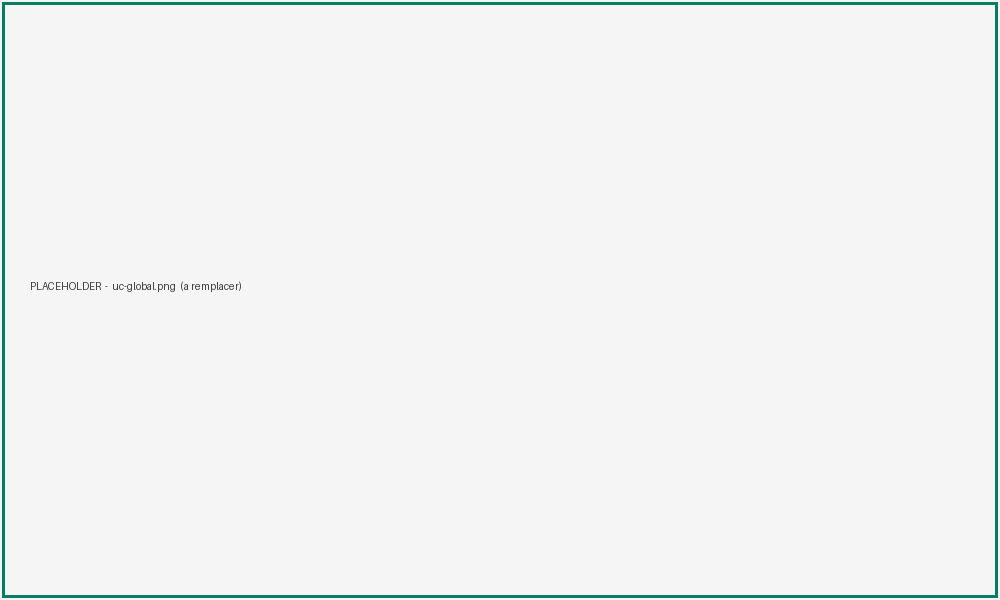
\includegraphics[width=0.9\linewidth]{images/uc-global.png} % À FOURNIR
  \caption{Diagramme de cas d'utilisation global}
  \label{fig:uc-global}
\end{figure}

\subsection{Description des cas d'utilisation principaux}

\paragraph{CU-01 : Rechercher un bien sur la carte.}
\begin{table}[H]
\centering
\renewcommand{\arraystretch}{1.2}
\begin{tabularx}{\linewidth}{>{\bfseries}p{2.8cm} X}
\toprule
Acteur         & Visiteur \\
Pré-condition  & La page de recherche cartographique est ouverte. \\
Scénario nominal &
1.~L'acteur déplace / zoome la carte.\newline
2.~Le système renvoie les biens situés dans l'emprise visible.\newline
3.~Les marqueurs sont affichés (regroupés si nombreux).\newline
4.~L'acteur clique un marqueur, consulte l'aperçu, puis ouvre la fiche. \\
Alternative    & 2a.~Aucun bien dans l'emprise~: message « aucun résultat ». \\
Post-condition & Liste et carte synchronisées sur la zone visible. \\
\bottomrule
\end{tabularx}
\caption{CU-01 « Rechercher un bien sur la carte »}
\label{tab:cu-recherche-carte}
\end{table}

\paragraph{CU-02 : Publier une annonce géolocalisée.}
\begin{table}[H]
\centering
\renewcommand{\arraystretch}{1.2}
\begin{tabularx}{\linewidth}{>{\bfseries}p{2.8cm} X}
\toprule
Acteur         & Particulier (ou Agent) \\
Pré-condition  & L'acteur est authentifié. \\
Scénario nominal &
1.~Saisie des caractéristiques du bien (type, prix, surface\ldots).\newline
2.~Choix du gouvernorat, de la délégation et de la localité.\newline
3.~Placement d'un marqueur sur la carte~; géocodage inverse et pré-remplissage
de l'adresse.\newline
4.~Ajout et réordonnancement des photos.\newline
5.~Soumission~; l'annonce passe à l'état « en attente ». \\
Alternative    & 5a.~Champs obligatoires manquants~: signalement des erreurs. \\
Post-condition & Une annonce en attente de modération est créée. \\
\bottomrule
\end{tabularx}
\caption{CU-02 « Publier une annonce géolocalisée »}
\label{tab:cu-publier}
\end{table}

\paragraph{CU-03 : Modérer une annonce.}
\begin{table}[H]
\centering
\renewcommand{\arraystretch}{1.2}
\begin{tabularx}{\linewidth}{>{\bfseries}p{2.8cm} X}
\toprule
Acteur         & Administrateur \\
Pré-condition  & Au moins une annonce est « en attente ». \\
Scénario nominal &
1.~Consultation de la file de modération.\newline
2.~Vérification du contenu, des photos et de la localisation.\newline
3.~Approbation~: l'annonce devient publique. \\
Alternative    & 3a.~Refus avec un ou plusieurs motifs et un message~; l'auteur
est notifié. \\
Post-condition & État de l'annonce~: « approuvée » ou « refusée ». \\
\bottomrule
\end{tabularx}
\caption{CU-03 « Modérer une annonce »}
\label{tab:cu-moderer}
\end{table}

\section*{Conclusion}
Les concepts clés, la solution et la spécification des besoins sont posés. Le
chapitre suivant traduit ces besoins en conception détaillée.


\chapter{Conception et modélisation}
\label{chap:conception}
% ===================== CHAPITRE 3 : CONCEPTION ET MODÉLISATION =====================

\section*{Introduction}
Ce chapitre constitue le cœur du travail~: architecture logique du système,
modélisation dynamique (séquence, activité), modélisation statique (classes) et
conception de la base de données (MCD, MLD, dictionnaire de données, règles de
gestion, normalisation).

\section{Architecture logique du système}
\label{sec:archi-logicielle}

Le système est conçu en couches, séparant la présentation, la logique
applicative et la persistance.

\begin{table}[H]
\centering
\renewcommand{\arraystretch}{1.25}
\begin{tabularx}{\linewidth}{>{\bfseries}p{3.2cm} X}
\toprule
Couche & Responsabilités \\
\midrule
Présentation      & Rendu des vues, carte interactive, formulaires, navigation. \\
Application (API) & Accès aux ressources, validation, contrôle d'accès par rôle, règles métier. \\
Accès aux données & Correspondance objets $\leftrightarrow$ tables, requêtes, transactions. \\
Persistance (SGBD) & Stockage relationnel, intégrité référentielle, index. \\
Services externes & Fond de carte et géocodage (OpenStreetMap). \\
\bottomrule
\end{tabularx}
\caption{Découpage en couches}
\label{tab:couches}
\end{table}

Les ressources manipulées sont~: \emph{utilisateurs}, \emph{annonces},
\emph{biens} (localisation), \emph{images}, \emph{référentiel géographique}
(gouvernorat, délégation, localité), \emph{favoris}, \emph{recherches
sauvegardées}. Le référentiel géographique est exposé sous forme de listes
dépendantes~: les délégations d'un gouvernorat, puis les localités d'une
délégation, avec une recherche textuelle de lieu retournant le niveau trouvé et
ses parents.

\section{Modélisation dynamique}
\label{sec:dynamique}

\subsection{Diagramme de séquence : recherche cartographique}
\begin{figure}[H]
  \centering
  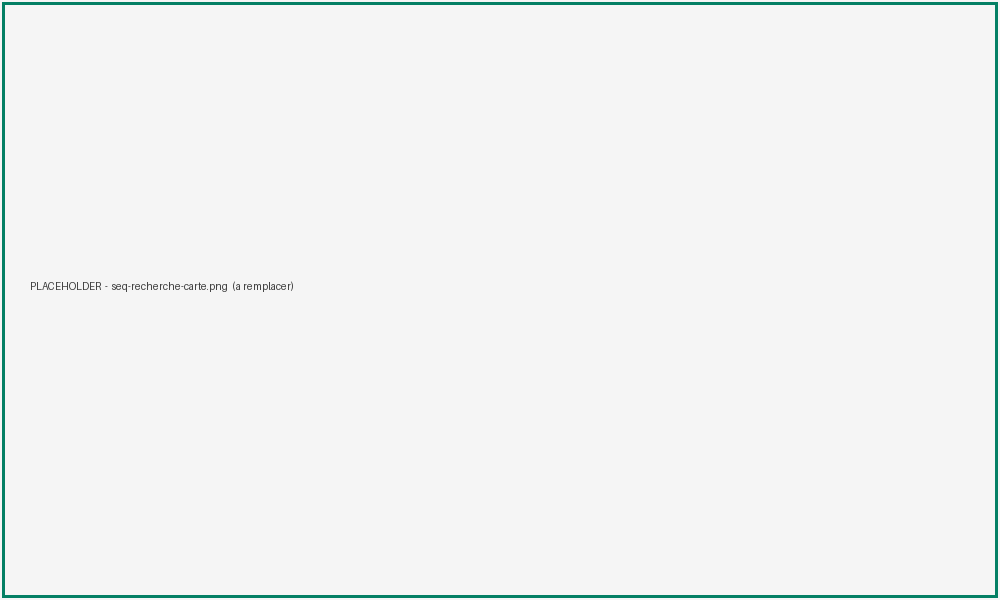
\includegraphics[width=0.9\linewidth]{images/seq-recherche-carte.png} % À FOURNIR
  \caption{Séquence « Rechercher un bien sur la carte »}
  \label{fig:seq-recherche}
\end{figure}
\noindent Le client transmet l'emprise courante de la carte~; le système renvoie
les biens dont les coordonnées appartiennent à cette emprise et dont l'annonce
est approuvée~; le client place les marqueurs et applique le regroupement.

\subsection{Diagramme de séquence : publication d'une annonce géolocalisée}
\begin{figure}[H]
  \centering
  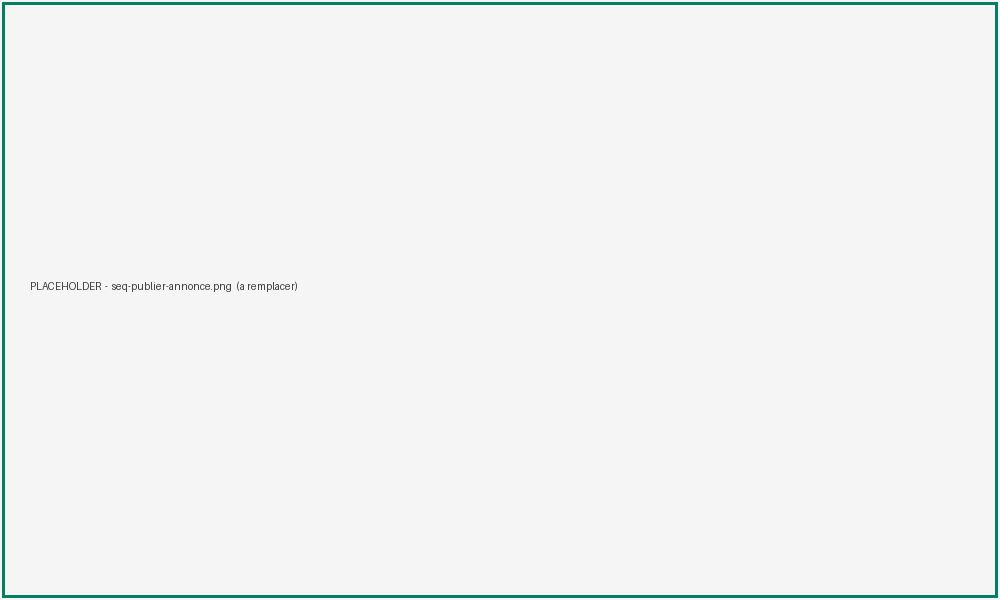
\includegraphics[width=0.9\linewidth]{images/seq-publier-annonce.png} % À FOURNIR
  \caption{Séquence « Publier une annonce géolocalisée »}
  \label{fig:seq-publier}
\end{figure}
\noindent Points remarquables~: (i) au dépôt du marqueur, un \textbf{géocodage
inverse} propose une adresse~; (ii) à la soumission, le système crée
l'\texttt{Annonce}, le \texttt{Bien} associé (relation 1--1) et ses images~;
(iii) l'annonce est créée à l'état \texttt{en attente}.

\subsection{Diagramme d'activité : cycle de vie d'une annonce}
\begin{figure}[H]
  \centering
  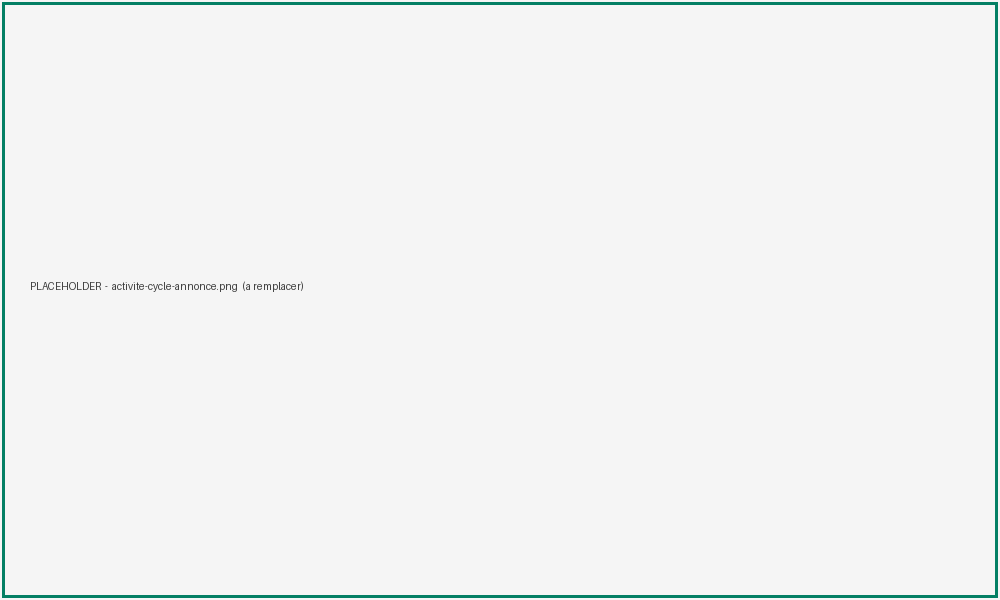
\includegraphics[width=0.62\linewidth]{images/activite-cycle-annonce.png} % À FOURNIR
  \caption{Cycle de vie d'une annonce (en attente, approuvée, refusée, vendue, louée)}
  \label{fig:cycle-annonce}
\end{figure}

\section{Modélisation statique : diagramme de classes}
\label{sec:classes}

\begin{figure}[H]
  \centering
  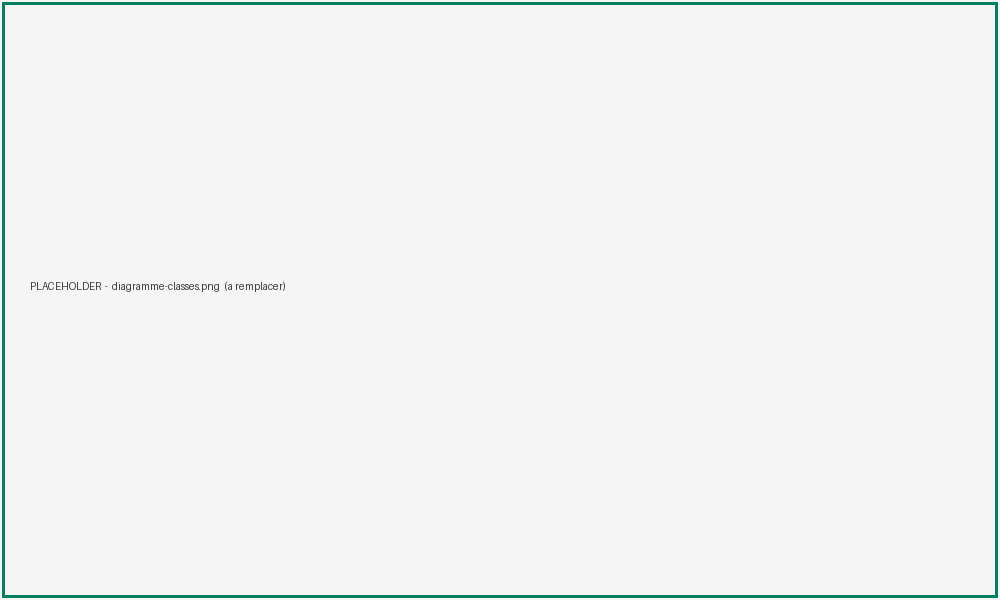
\includegraphics[width=\linewidth]{images/diagramme-classes.png} % À FOURNIR
  \caption{Diagramme de classes du domaine}
  \label{fig:classes}
\end{figure}

\begin{table}[H]
\centering
\renewcommand{\arraystretch}{1.2}
\begin{tabularx}{\linewidth}{>{\bfseries}p{3.1cm} X}
\toprule
Classe & Rôle \\
\midrule
\texttt{Utilisateur} & Compte de la plateforme~; porte le rôle (particulier, agent, agence, promoteur, administrateur) et le profil. \\
\texttt{Agence}       & Entité professionnelle rattachée à un utilisateur~; regroupe des agents. \\
\texttt{Annonce}      & Offre de vente / location / vacances d'un bien~; porte l'état de modération, le prix, les caractéristiques générales. \\
\texttt{Bien}         & Localisation~: adresse, latitude, longitude, image principale~; relation 1--1 avec \texttt{Annonce}. \\
\texttt{Image}        & Photo d'un bien, avec un ordre d'affichage. \\
\texttt{Gouvernorat}, \texttt{Delegation}, \texttt{Localite} & Référentiel géographique hiérarchique. \\
\texttt{Favori}       & Association \texttt{Utilisateur}--\texttt{Annonce} (bien enregistré). \\
\texttt{RechercheSauvegardee} & Critères de recherche d'un utilisateur + alerte. \\
\bottomrule
\end{tabularx}
\caption{Classes principales du modèle}
\label{tab:classes-principales}
\end{table}

\paragraph{Associations et multiplicités.}
\begin{itemize}[label=\textbullet,itemsep=1pt]
  \item \texttt{Utilisateur} \emph{1} --- \emph{0..*} \texttt{Annonce}~;
  \item \texttt{Annonce} \emph{1} --- \emph{1} \texttt{Bien}~;
        \texttt{Bien} \emph{1} --- \emph{0..*} \texttt{Image}~;
  \item \texttt{Gouvernorat} \emph{1} --- \emph{0..*} \texttt{Delegation}
        \emph{1} --- \emph{0..*} \texttt{Localite}~;
  \item \texttt{Annonce} \emph{*} --- \emph{1} de chacun de
        \texttt{Gouvernorat}, \texttt{Delegation}, \texttt{Localite}~;
  \item \texttt{Utilisateur} \emph{*} --- \emph{*} \texttt{Annonce} via
        \texttt{Favori}~;
  \item \texttt{Agence} \emph{1} --- \emph{0..*} \texttt{Utilisateur} (agents).
\end{itemize}

\paragraph{Énumérations du domaine.}
\begin{table}[H]
\centering
\renewcommand{\arraystretch}{1.15}
\begin{tabularx}{\linewidth}{>{\bfseries}p{3cm} X}
\toprule
Énumération & Valeurs (extrait) \\
\midrule
Rôle          & admin, promoteur, agence, agent, particulier \\
Catégorie     & vente, location, vacances \\
Type de bien  & appartement, duplex, penthouse, villa, bureau, local commercial, terrain, ferme agricole, immeuble, garage/parking \\
État du bien  & nouveau, bon état, à rénover, en cours de construction \\
Statut d'annonce & en attente, approuvée, refusée, vendue, louée \\
Devise        & DT, EUR, USD \\
\bottomrule
\end{tabularx}
\caption{Principales énumérations}
\label{tab:enums}
\end{table}

\section{Conception de la base de données}
\label{sec:bdd}

\subsection{Choix du SGBD}
Le choix se porte sur un SGBD \textbf{relationnel} (PostgreSQL) pour l'intégrité
référentielle et le typage riche (numérique décimal pour les prix, énumérations,
dates), avec la possibilité d'une extension spatiale (PostGIS) si des requêtes
géographiques avancées (recherche par rayon, distance) deviennent nécessaires.

\subsection{Modèle conceptuel de données (MCD)}
\begin{figure}[H]
  \centering
  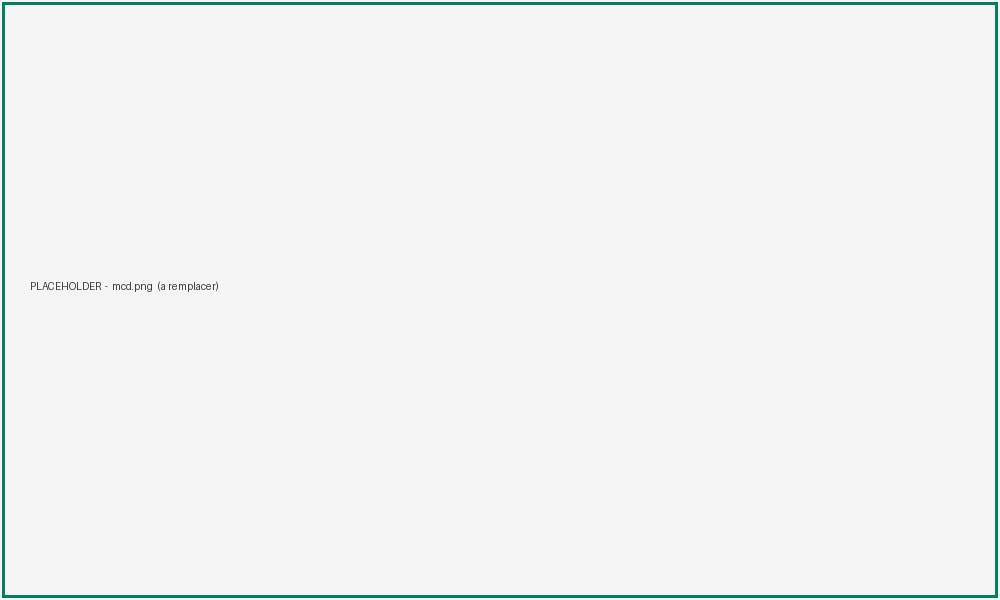
\includegraphics[width=\linewidth]{images/mcd.png} % À FOURNIR (Looping / draw.io)
  \caption{Modèle conceptuel de données}
  \label{fig:mcd}
\end{figure}
\noindent Le triplet géographique modélise une hiérarchie stricte sans cycle~;
l'entité \textsc{Bien} porte les coordonnées~; l'adresse administrative d'une
annonce est \emph{référencée} et non dupliquée.

\subsection{Modèle logique de données (MLD)}
Clés primaires soulignées, clés étrangères en italique.

\begin{longtable}{p{3.2cm} p{10.3cm}}
\caption{Modèle logique de données (extrait)}\label{tab:mld}\\
\toprule
\textbf{Relation} & \textbf{Attributs} \\
\midrule
\endfirsthead
\toprule
\textbf{Relation} & \textbf{Attributs} \\
\midrule
\endhead
users        & \underline{id}, username, email, mot\_de\_passe, role, telephone, nom, prenom, nom\_entreprise, \textit{agence\_id}, gouvernorat, localite, date\_creation \\
agencies     & \underline{id}, \textit{user\_id}, nom, email, telephone, adresse, matricule, reference, date\_creation \\
gouvernorats & \underline{id}, nom \\
delegations  & \underline{id}, nom, \textit{gouvernorat\_id} \\
localites    & \underline{id}, nom, \textit{delegation\_id} \\
annonces     & \underline{id}, reference, \textit{utilisateur\_id}, \textit{gouvernorat\_id}, \textit{delegation\_id}, \textit{localite\_id}, categorie, type\_bien, etat\_bien, titre, description, superficie, prix, devise, status, nb\_pieces, nb\_chambres, nb\_salles\_bain, date\_creation, date\_mise\_a\_jour \\
biens        & \underline{id}, \textit{annonce\_id} (unique), adresse, latitude, longitude, image\_principale \\
images       & \underline{id}, \textit{bien\_id}, url, ordre \\
favoris      & \underline{id}, \textit{user\_id}, \textit{annonce\_id}, date \; -- \; UNIQUE(user\_id, annonce\_id) \\
recherches\_sauvegardees & \underline{id}, \textit{user\_id}, nom, criteres, alerte\_email, date \\
\bottomrule
\end{longtable}

\subsection{Dictionnaire de données}
\begin{longtable}{p{2.8cm} p{2.5cm} p{2cm} p{5.4cm}}
\caption{Dictionnaire de données (tables centrales)}\label{tab:dictionnaire}\\
\toprule
\textbf{Attribut} & \textbf{Type} & \textbf{Contraintes} & \textbf{Description} \\
\midrule
\endfirsthead
\toprule
\textbf{Attribut} & \textbf{Type} & \textbf{Contraintes} & \textbf{Description} \\
\midrule
\endhead
\multicolumn{4}{l}{\textit{Table \texttt{annonces}}}\\
id            & entier        & PK, auto       & Identifiant annonce \\
reference     & chaîne        & unique         & Référence lisible (ex. TN0001) \\
utilisateur\_id & entier      & FK users.id    & Auteur de l'annonce \\
gouvernorat\_id & entier      & FK             & Gouvernorat \\
delegation\_id & entier       & FK             & Délégation \\
localite\_id  & entier        & FK             & Localité \\
categorie     & énum          & non nul        & vente / location / vacances \\
type\_bien    & énum          & non nul        & Type de bien \\
etat\_bien    & énum          &                & État du bien \\
titre         & chaîne        & non nul        & Titre de l'annonce \\
superficie    & réel          &                & Surface en m\textsuperscript{2} \\
prix          & décimal(12,2) & $>$ 0          & Prix \\
devise        & énum          & défaut DT      & Devise \\
status        & énum          & défaut en attente & État de modération \\
date\_creation & horodatage   & défaut \emph{now} & Date de dépôt \\
\midrule
\multicolumn{4}{l}{\textit{Table \texttt{biens}}}\\
id            & entier        & PK, auto       & Identifiant du bien \\
annonce\_id   & entier        & FK, \textbf{unique} & Annonce associée (1--1) \\
adresse       & chaîne        &                & Adresse lisible (géocodage inverse) \\
latitude      & réel          &                & Latitude WGS 84 (degrés décimaux) \\
longitude     & réel          &                & Longitude WGS 84 (degrés décimaux) \\
image\_principale & chaîne    & nullable       & URL de l'aperçu \\
\midrule
\multicolumn{4}{l}{\textit{Tables \texttt{gouvernorats} / \texttt{delegations} / \texttt{localites}}}\\
id            & entier        & PK, auto       & Identifiant \\
nom           & chaîne        & non nul        & Libellé \\
gouvernorat\_id & entier      & FK (delegations) & Gouvernorat parent \\
delegation\_id & entier       & FK (localites)  & Délégation parente \\
\bottomrule
\end{longtable}

\subsection{Règles de gestion}
\begin{enumerate}[label=RG-\arabic*.,itemsep=1pt]
  \item Une annonce appartient à un et un seul utilisateur.
  \item Une annonce décrit exactement un bien, et réciproquement (relation 1--1
        garantie par l'unicité de \texttt{annonce\_id} dans \texttt{biens}).
  \item Une localité appartient à une délégation, une délégation à un
        gouvernorat~; la hiérarchie ne comporte pas de cycle.
  \item Le triplet (gouvernorat, délégation, localité) d'une annonce est
        cohérent avec la hiérarchie.
  \item Les coordonnées doivent être situées dans l'emprise de la Tunisie
        (contrôle applicatif).
  \item Une annonce est créée à l'état « en attente »~; seul un administrateur
        la fait passer à « approuvée » ou « refusée ».
  \item Un refus est accompagné d'au moins un motif.
  \item Un utilisateur ne peut mettre une même annonce en favori qu'une fois.
  \item Le prix est strictement positif, dans une devise du catalogue.
  \item Un agent est rattaché à au plus une agence.
\end{enumerate}

\subsection{Normalisation}
Le schéma respecte la troisième forme normale~: attributs atomiques (les photos
sont externalisées dans \texttt{images})~; clé primaire technique simple sur
chaque table (pas de dépendance partielle)~; pas de dépendance transitive
(l'adresse administrative est référencée via des clés étrangères, non
recopiée).

\section*{Conclusion}
La conception du système est établie~: architecture en couches, diagrammes de
séquence et d'activité, diagramme de classes, et conception complète de la base
de données. Le chapitre suivant traite de la conception des interfaces
utilisateur.


\chapter{Conception des interfaces utilisateur}
\label{chap:uxui}
% ===================== CHAPITRE 4 : CONCEPTION DES INTERFACES UTILISATEUR =====================

\section*{Introduction}
Ce chapitre décrit la conception des interfaces selon une démarche centrée
utilisateur~: personas et parcours, architecture de l'information, wireframes,
charte graphique, puis maquettes et prototype interactif réalisés sous
\textbf{Figma}.

\section{Démarche et outils}
\label{sec:demarche-ux}
La conception suit un processus itératif~: \textbf{comprendre} (besoins,
existant), \textbf{définir} (personas, parcours), \textbf{structurer}
(arborescence, wireframes), \textbf{maquetter} (charte, maquettes haute
fidélité), \textbf{prototyper} (enchaînement des écrans). L'outil retenu est
\textbf{Figma}, pour le travail collaboratif, la bibliothèque de composants
réutilisables et le mode prototype.

\section{Personas et parcours}
\label{sec:personas}

\begin{table}[H]
\centering
\renewcommand{\arraystretch}{1.25}
\begin{tabularx}{\linewidth}{>{\bfseries}p{3cm} X}
\toprule
Persona & Besoin principal \\
\midrule
Amine, 29 ans, locataire & Trouver un appartement proche de son travail~; usage mobile~; carte + filtres budget/quartier. \\
Sonia, 41 ans, propriétaire & Publier facilement sa villa~; positionner précisément le bien~; gérer les photos. \\
Karim, 35 ans, agent & Saisie rapide de nombreuses annonces~; espace dédié et tableau de bord. \\
Leïla, administratrice & File de modération claire~; vérification de la localisation~; motifs de refus normalisés. \\
\bottomrule
\end{tabularx}
\caption{Personas}
\label{tab:personas}
\end{table}

\begin{figure}[H]
  \centering
  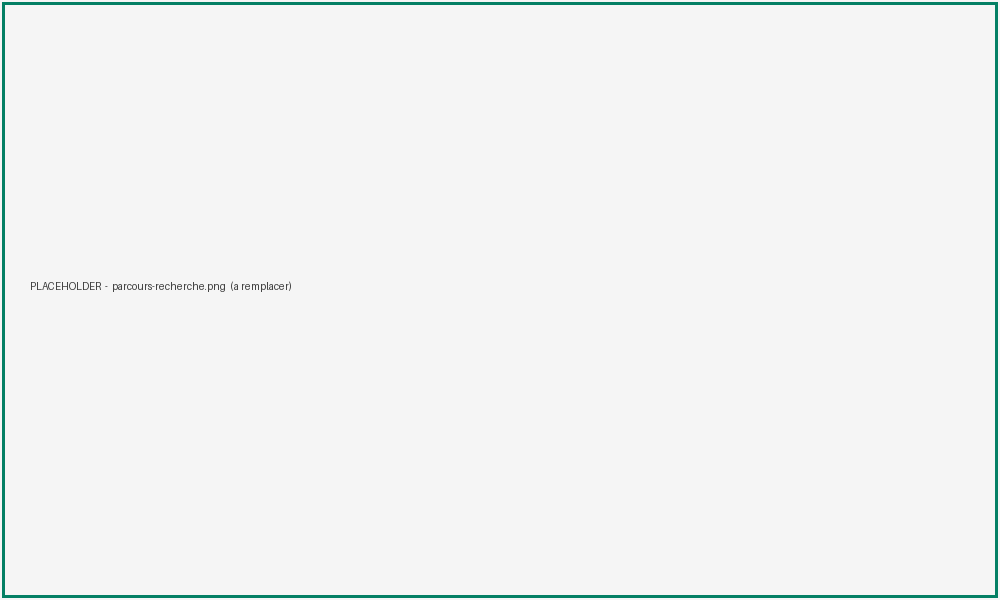
\includegraphics[width=0.9\linewidth]{images/parcours-recherche.png} % À FOURNIR (Figma)
  \caption{Parcours utilisateur « rechercher et contacter »}
  \label{fig:parcours-recherche}
\end{figure}
\noindent Étapes~: accueil $\rightarrow$ saisie d'un lieu ou géolocalisation
$\rightarrow$ carte + liste $\rightarrow$ affinage des filtres $\rightarrow$
fiche détaillée $\rightarrow$ favori / comparaison $\rightarrow$ contact.

\section{Architecture de l'information}
\label{sec:arbo}

\begin{figure}[H]
  \centering
  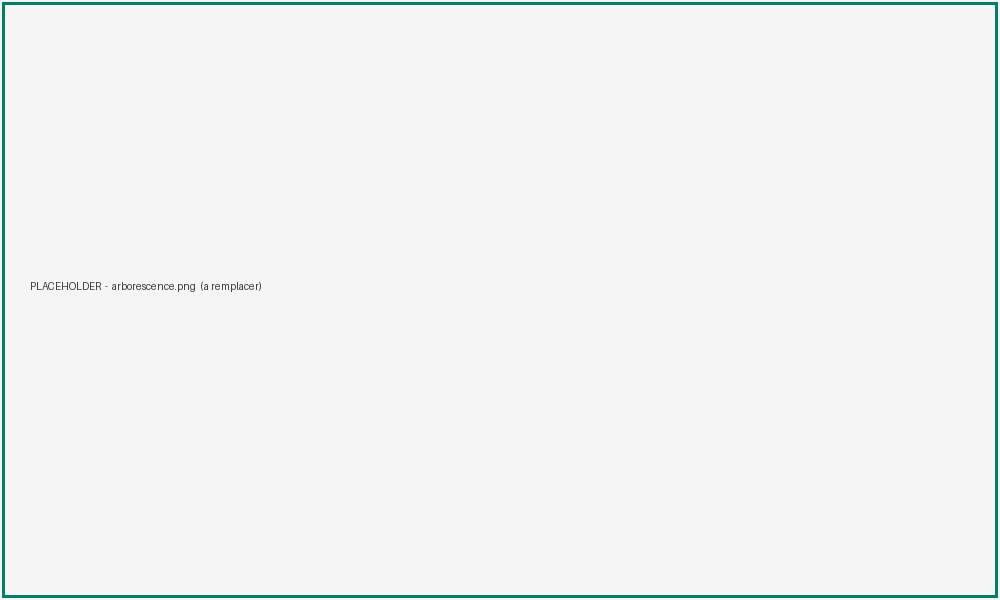
\includegraphics[width=0.92\linewidth]{images/arborescence.png} % À FOURNIR (Figma)
  \caption{Arborescence (plan de site)}
  \label{fig:arborescence}
\end{figure}

\begin{table}[H]
\centering
\renewcommand{\arraystretch}{1.2}
\begin{tabularx}{\linewidth}{>{\bfseries}p{3.2cm} X}
\toprule
Zone & Écrans \\
\midrule
Public        & Accueil, Recherche (liste), Recherche sur carte, Détail d'une annonce, Comparateur, Contenus (À propos, FAQ, Contact). \\
Compte        & Connexion, Inscription, Mot de passe oublié, Mon compte, Mes favoris, Mes recherches. \\
Publication   & Assistant « Créer une annonce » (multi-étapes), Modifier une annonce. \\
Professionnel & Espace agence (portefeuille, agents, tableau de bord). \\
Administration & Tableau de bord admin, modération des annonces, gestion des comptes. \\
\bottomrule
\end{tabularx}
\caption{Regroupement des écrans}
\label{tab:pages}
\end{table}

\noindent La navigation repose sur une barre persistante (logo, recherche,
« Publier », compte), une bascule \textbf{Liste $\leftrightarrow$ Carte} toujours
accessible, et un menu utilisateur contextuel selon le rôle.

\section{Wireframes (basse fidélité)}
\label{sec:wireframes}

\begin{figure}[H]
  \centering
  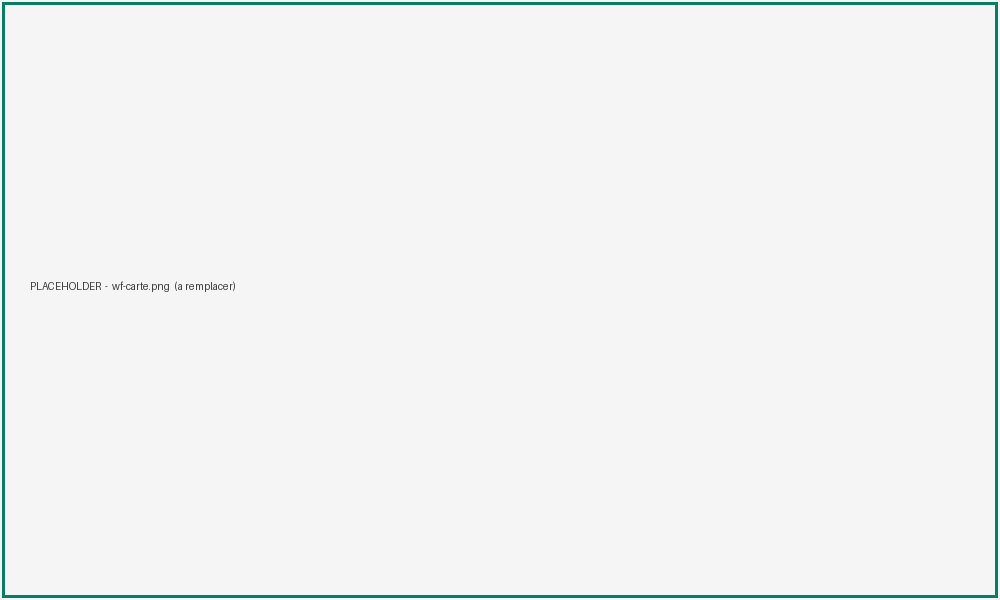
\includegraphics[width=0.9\linewidth]{images/wf-carte.png} % À FOURNIR (Figma)
  \caption{Wireframe : recherche sur carte}
  \label{fig:wf-carte}
\end{figure}
\noindent Colonne de filtres repliable, carte plein écran avec marqueurs
regroupés, panneau de résultats synchronisé avec l'emprise (survol croisé
carte $\leftrightarrow$ liste).

\begin{figure}[H]
  \centering
  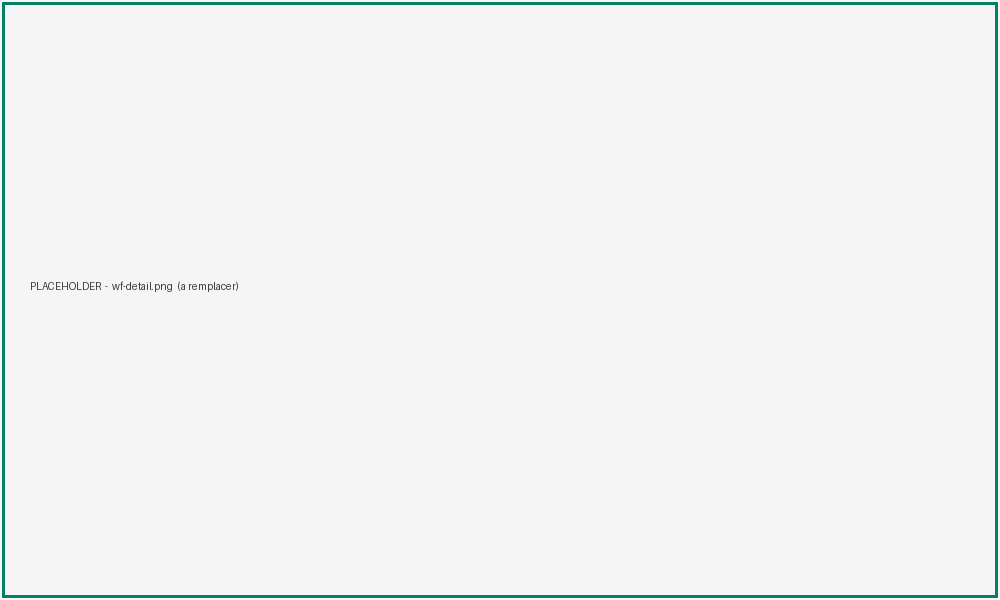
\includegraphics[width=0.9\linewidth]{images/wf-detail.png} % À FOURNIR (Figma)
  \caption{Wireframe : détail d'une annonce}
  \label{fig:wf-detail}
\end{figure}
\noindent Blocs~: galerie photos, titre + prix + localisation, caractéristiques,
description, \textbf{carte de situation}, équipements, bloc contact, biens
similaires.

\begin{figure}[H]
  \centering
  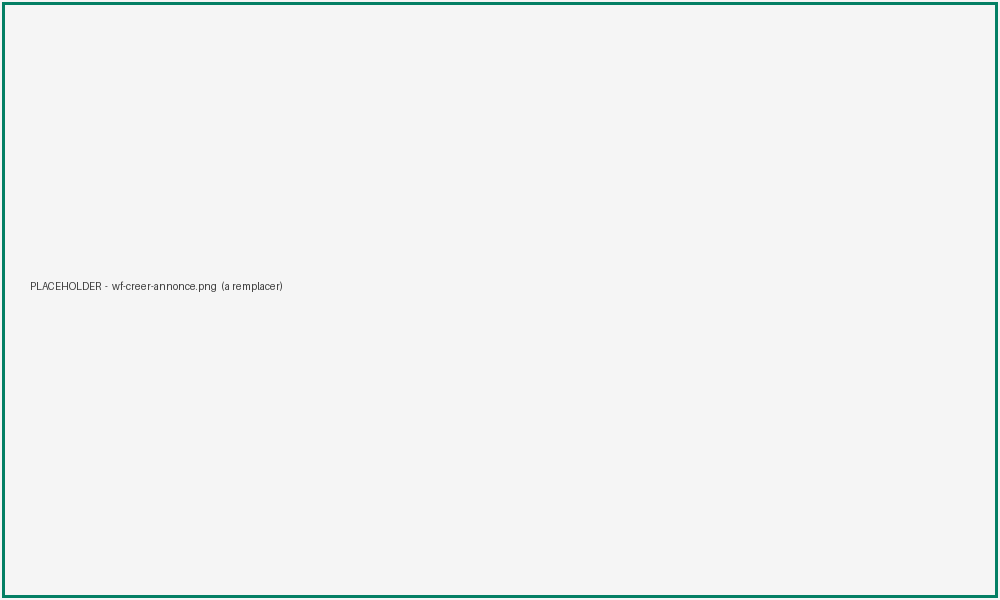
\includegraphics[width=0.9\linewidth]{images/wf-creer-annonce.png} % À FOURNIR (Figma)
  \caption{Wireframe : assistant « Créer une annonce »}
  \label{fig:wf-creer}
\end{figure}
\noindent Étapes~: (1) catégorie et type~; (2) caractéristiques~;
(3) \textbf{localisation} (référentiel + placement sur carte + géocodage
inverse)~; (4) photos (glisser-déposer)~; (5) prix et options~;
(6) récapitulatif et soumission~; une barre de progression indique l'étape.

\begin{figure}[H]
  \centering
  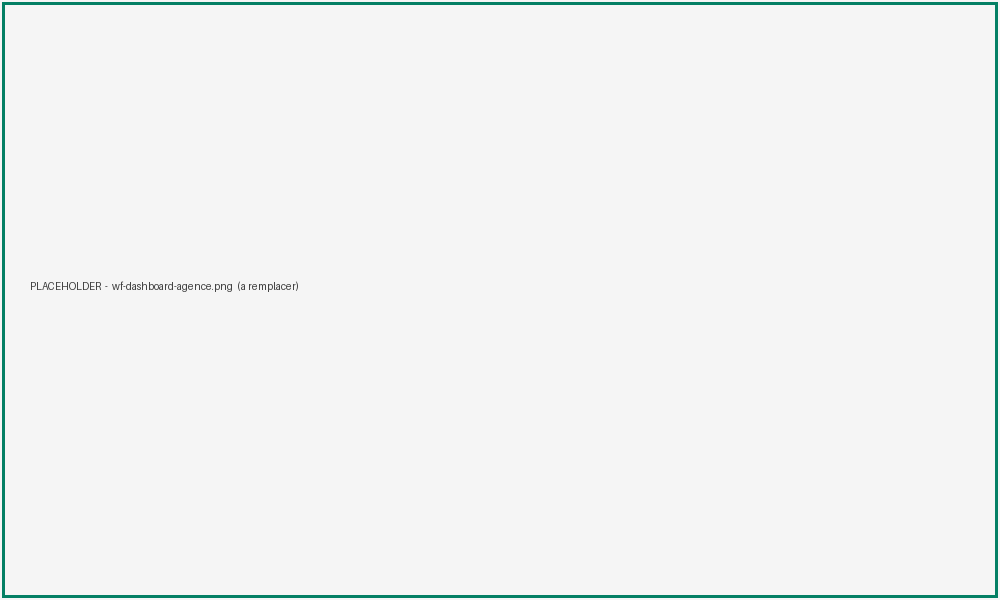
\includegraphics[width=0.9\linewidth]{images/wf-dashboard-agence.png} % À FOURNIR (Figma)
  \caption{Wireframe : tableau de bord agence}
  \label{fig:wf-dashboard}
\end{figure}

\section{Charte graphique}
\label{sec:charte}

\begin{table}[H]
\centering
\renewcommand{\arraystretch}{1.25}
\begin{tabularx}{\linewidth}{>{\bfseries}p{3cm} p{3cm} X}
\toprule
Rôle & Code (exemple) & Usage \\
\midrule
Primaire   & \texttt{\#047F64} & Actions principales, liens, marqueurs actifs. \\
Secondaire & \texttt{\#0077B6} & Accents, éléments d'information. \\
Accent     & \texttt{\#ED6E0A} & Mises en avant, badges. \\
Fond neutre & \texttt{\#F5F5F5} & Arrière-plans de sections. \\
Texte      & \texttt{\#1F2937} & Corps de texte. \\
Succès / Erreur & \texttt{\#16A34A} / \texttt{\#DC2626} & États de validation. \\
\bottomrule
\end{tabularx}
\caption{Palette de couleurs (à valider avec la charte de l'organisme)}
\label{tab:palette}
\end{table}

\noindent \textbf{Typographie}~: police sans empattement lisible à l'écran
(ex.~\emph{Inter} / \emph{Poppins})~; hiérarchie H1--H3, corps 16~px, légendes
13~px~; interlignage 1,5.
\textbf{Composants Figma}~: boutons, champs, listes déroulantes dépendantes
(gouvernorat $\rightarrow$ délégation $\rightarrow$ localité), cartes de bien,
marqueurs et \emph{popups}, fenêtres modales, \emph{toasts}, barre de
progression, pagination.
\textbf{Rendu cartographique}~: marqueur standard, marqueur mis en avant,
marqueur sélectionné~; pastille numérotée pour le regroupement~; \emph{popup} au
clic (photo, prix, titre, lien vers la fiche).

\section{Maquettes haute fidélité et prototype}
\label{sec:maquettes}

\begin{figure}[H]
  \centering
  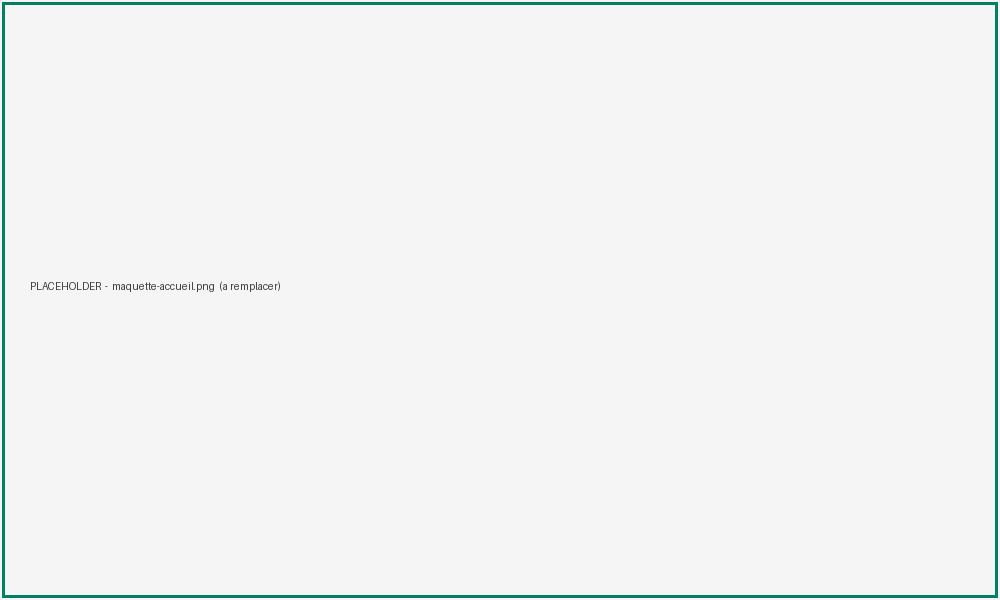
\includegraphics[width=0.9\linewidth]{images/maquette-accueil.png} % À FOURNIR (Figma)
  \caption{Maquette haute fidélité : page d'accueil}
  \label{fig:maquette-accueil}
\end{figure}

\begin{figure}[H]
  \centering
  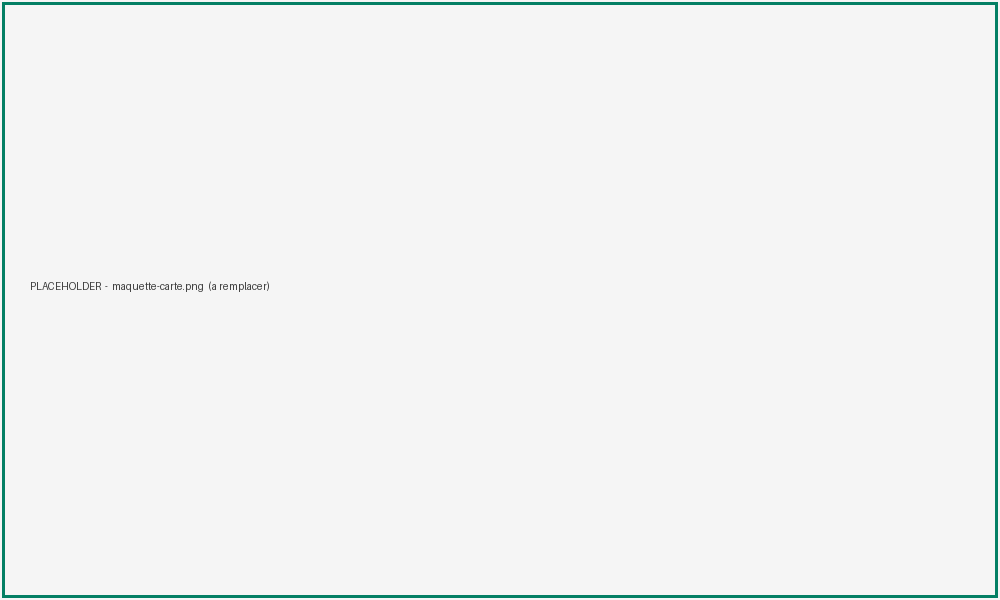
\includegraphics[width=0.9\linewidth]{images/maquette-carte.png} % À FOURNIR (Figma)
  \caption{Maquette haute fidélité : recherche sur carte}
  \label{fig:maquette-carte}
\end{figure}

\begin{figure}[H]
  \centering
  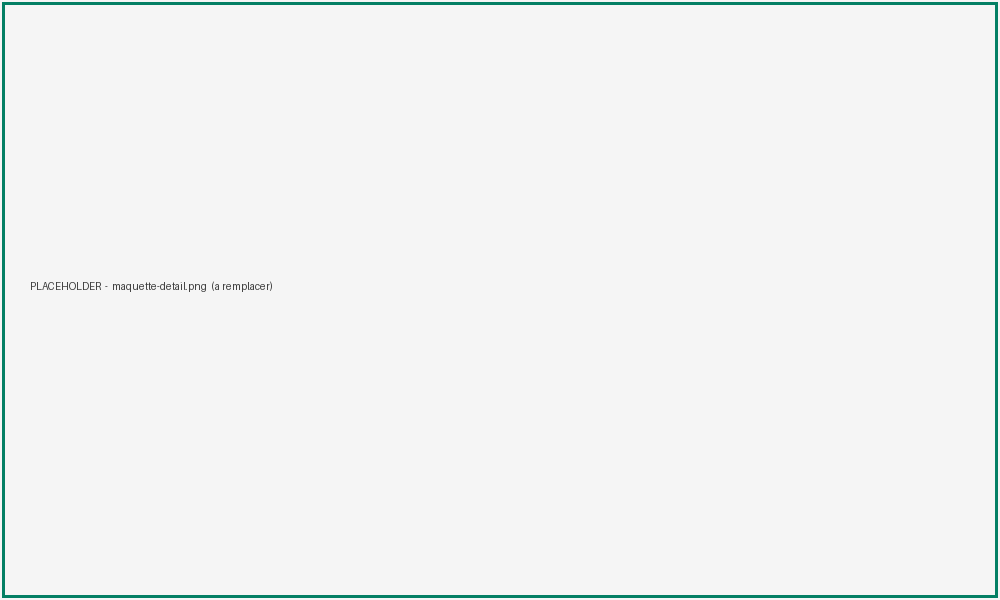
\includegraphics[width=0.9\linewidth]{images/maquette-detail.png} % À FOURNIR (Figma)
  \caption{Maquette haute fidélité : détail d'une annonce}
  \label{fig:maquette-detail}
\end{figure}

\noindent Les écrans sont reliés dans le \textbf{mode prototype de Figma} pour
simuler les parcours principaux (recherche, publication, modération) et valider
l'enchaînement des interactions avant tout développement. Lien du prototype~:
[\ldots].

\section{Ergonomie et accessibilité}
\label{sec:accessibilite}
\begin{itemize}[label=\textbullet,itemsep=1pt]
  \item respect des heuristiques de Nielsen (retour d'information, prévention des
        erreurs, cohérence, contrôle utilisateur)~;
  \item conformité visée \textbf{WCAG 2.1 niveau AA}~: contrastes suffisants,
        navigation clavier, libellés de formulaire explicites, textes
        alternatifs, cibles tactiles $\geq$ 44~px~;
  \item conception \textbf{responsive} (points de rupture indicatifs 360, 768,
        1024, 1280~px)~; filtres et liste en tiroirs sur mobile.
\end{itemize}

\section*{Conclusion}
La conception des interfaces est complète~: personas et parcours, arborescence,
wireframes, charte graphique, maquettes et prototype Figma. L'ensemble constitue
une base prête pour la phase de développement.


\chapter{Conclusion générale et perspectives}
\label{chap:conclusion}
% ===================== CONCLUSION GÉNÉRALE ET PERSPECTIVES =====================

\section{Bilan}

Ce projet a porté sur la \textbf{conception et la modélisation} d'une plateforme
web de \textbf{géolocalisation des biens immobiliers en Tunisie}. Le travail,
volontairement limité à la phase amont, a permis de~:

\begin{itemize}[label=\textbullet,itemsep=1pt]
  \item analyser le contexte et l'existant, et formaliser un cahier des charges
        (besoins fonctionnels et non fonctionnels)~;
  \item définir une architecture logique en couches et identifier les acteurs et
        les cas d'utilisation~;
  \item réaliser la modélisation UML (cas d'utilisation, séquence, activité,
        classes)~;
  \item concevoir la base de données~: MCD, MLD, dictionnaire de données, règles
        de gestion, normalisation en 3FN, avec au centre le double adressage
        \emph{référentiel hiérarchique} (gouvernorat, délégation, localité)
        \emph{et coordonnées GPS}~;
  \item concevoir les interfaces sous Figma~: personas, parcours, arborescence,
        wireframes, charte graphique, maquettes haute fidélité et prototype
        interactif.
\end{itemize}

\section{Difficultés rencontrées}
\begin{itemize}[label=\textbullet,itemsep=1pt]
  \item concilier adressage administratif structuré et coordonnées exactes sans
        redondance ni incohérence~;
  \item garantir la lisibilité de la carte avec un grand nombre de biens
        (principe du regroupement de marqueurs)~;
  \item modéliser la diversité des types de biens et la variété des rôles métier.
\end{itemize}

\section{Perspectives}
\begin{itemize}[label=\textbullet,itemsep=1pt]
  \item \textbf{Développement} de la plateforme à partir de la présente
        conception~;
  \item recherche géographique avancée (rayon, itinéraires, points d'intérêt) via
        une extension spatiale~;
  \item recommandation de biens fondée sur l'historique et les recherches
        sauvegardées~;
  \item estimation automatique de prix à partir de la localisation et des
        caractéristiques~;
  \item visite virtuelle et modélisation 3D des biens.
\end{itemize}

\medskip
\noindent Ce travail fournit une base de conception documentée et cohérente pour
le développement complet de la plateforme.


% =================== BIBLIOGRAPHIE ===================
\begin{thebibliography}{99}
\setlength{\itemsep}{10pt}

\bibitem{ref:entreprise} Site de l'organisme d'accueil \rapportEntreprise, \url{https://exemple.tn/}, consulté en 2026. % À ADAPTER

\bibitem{ref:uml} OMG, \emph{Unified Modeling Language (UML) Specification}, version 2.5.1, Object Management Group, \url{https://www.omg.org/spec/UML/}.

\bibitem{ref:roques} P.~Roques, \emph{UML 2 par la pratique : études de cas et exercices corrigés}, Eyrolles.

\bibitem{ref:merise} D.~Nanci, B.~Espinasse, \emph{Ingénierie des systèmes d'information : Merise}, Vuibert.

\bibitem{ref:postgres} \emph{PostgreSQL Documentation}, The PostgreSQL Global Development Group, \url{https://www.postgresql.org/docs/}.

\bibitem{ref:postgis} \emph{PostGIS -- Spatial and Geographic Objects for PostgreSQL}, \url{https://postgis.net/}.

\bibitem{ref:leaflet} V.~Agafonkin, \emph{Leaflet -- an open-source JavaScript library for interactive maps}, \url{https://leafletjs.com/}.

\bibitem{ref:osm} \emph{OpenStreetMap}, \url{https://www.openstreetmap.org/}.

\bibitem{ref:nominatim} \emph{Nominatim -- Geocoding with OpenStreetMap data}, \url{https://nominatim.org/}.

\bibitem{ref:ins} Institut National de la Statistique (Tunisie), \emph{Découpage administratif : gouvernorats, délégations, secteurs}, \url{https://www.ins.tn/}.

\bibitem{ref:nielsen} J.~Nielsen, \emph{10 Usability Heuristics for User Interface Design}, Nielsen Norman Group, \url{https://www.nngroup.com/articles/ten-usability-heuristics/}.

\bibitem{ref:wcag} W3C, \emph{Web Content Accessibility Guidelines (WCAG) 2.1}, \url{https://www.w3.org/TR/WCAG21/}.

\bibitem{ref:figma} \emph{Figma -- The collaborative interface design tool}, \url{https://www.figma.com/}.

\end{thebibliography}

\end{document}
